\documentclass[oneside]{book}

\setcounter{tocdepth}{1}
\setcounter{secnumdepth}{3}

\usepackage[toc,page]{appendix}
\usepackage{hyperref}
\usepackage[utf8]{inputenc}
\usepackage{graphicx} % Required for the inclusion of images
\usepackage{amsmath} % Required for some math elements 
\usepackage[utf8]{inputenc}
\usepackage[english]{babel}
\newtheorem{theorem}{Theorem}
\newtheorem{corollary}{Corollary}[theorem]
\newtheorem{lemma}[theorem]{Lemma}
\usepackage{listings}
\usepackage{pdfpages}
\usepackage{amssymb}
\usepackage{pdflscape}

\begin{document}

\begin{titlepage}
	\centering
	
\includegraphics[width=0.60\textwidth]{../logo/UoN_Primary_Logo_RGB.png}\par\vspace{1cm}
	\vspace{1.5cm}
	{\huge\bfseries Terminology in Functional Agent-Based Simulation \par}
	\vspace{2cm}
	{\Large\itshape jonathan.thaler@nottingham.ac.uk \par}
	\vfill
	
	\vfill

	{\large \today\par}
\end{titlepage}

\cleardoublepage

\section*{Abstract}
This document is a collection of the used terminology for the thesis on Functional Agent-Based Simulation. It explains each term, its relevance to the field and the connections to other terms. Included is an A3 poster which visualizes all terms and their connections and can be seen as a mind-map as well.
The intention of this document and poster is to clarify the exact meaning of various terms, their implications and relations to others - to clarify my thinking and discussions.

% TODO: what about an "abstraction" hierarchy? e.g. in this field we have multiple abstraction-layers. e.g. layer 0 paradigms: functional vs. oop, layer 1 languages: haskell vs. java, layer 2 libraries: Yampa (FrABS) vs. Repast Simphony

\clearpage

\section*{Agent}

\section*{Actor}

\section*{Agent-Based Simulation (ABS)}

\section*{Agent-Based Modelling (ABM)}

\section*{Agent-Based Modelling \& Simulation (ABMS)}

\section*{Multi-Agent System (MAS)}

\section*{Agent-Based Social Simulation (ABSS)}

\section*{Agent-Based Computational Economics (ACE)}

\section*{Scala}

\section*{Erlang}

\section*{Haskell}

\section*{Functional Reactive Programming (FRP)}

\section*{Yampa}

\section*{Embedded Domain Specific Language (EDSL)}

\section*{Repast Simphony}

\begin{landscape}
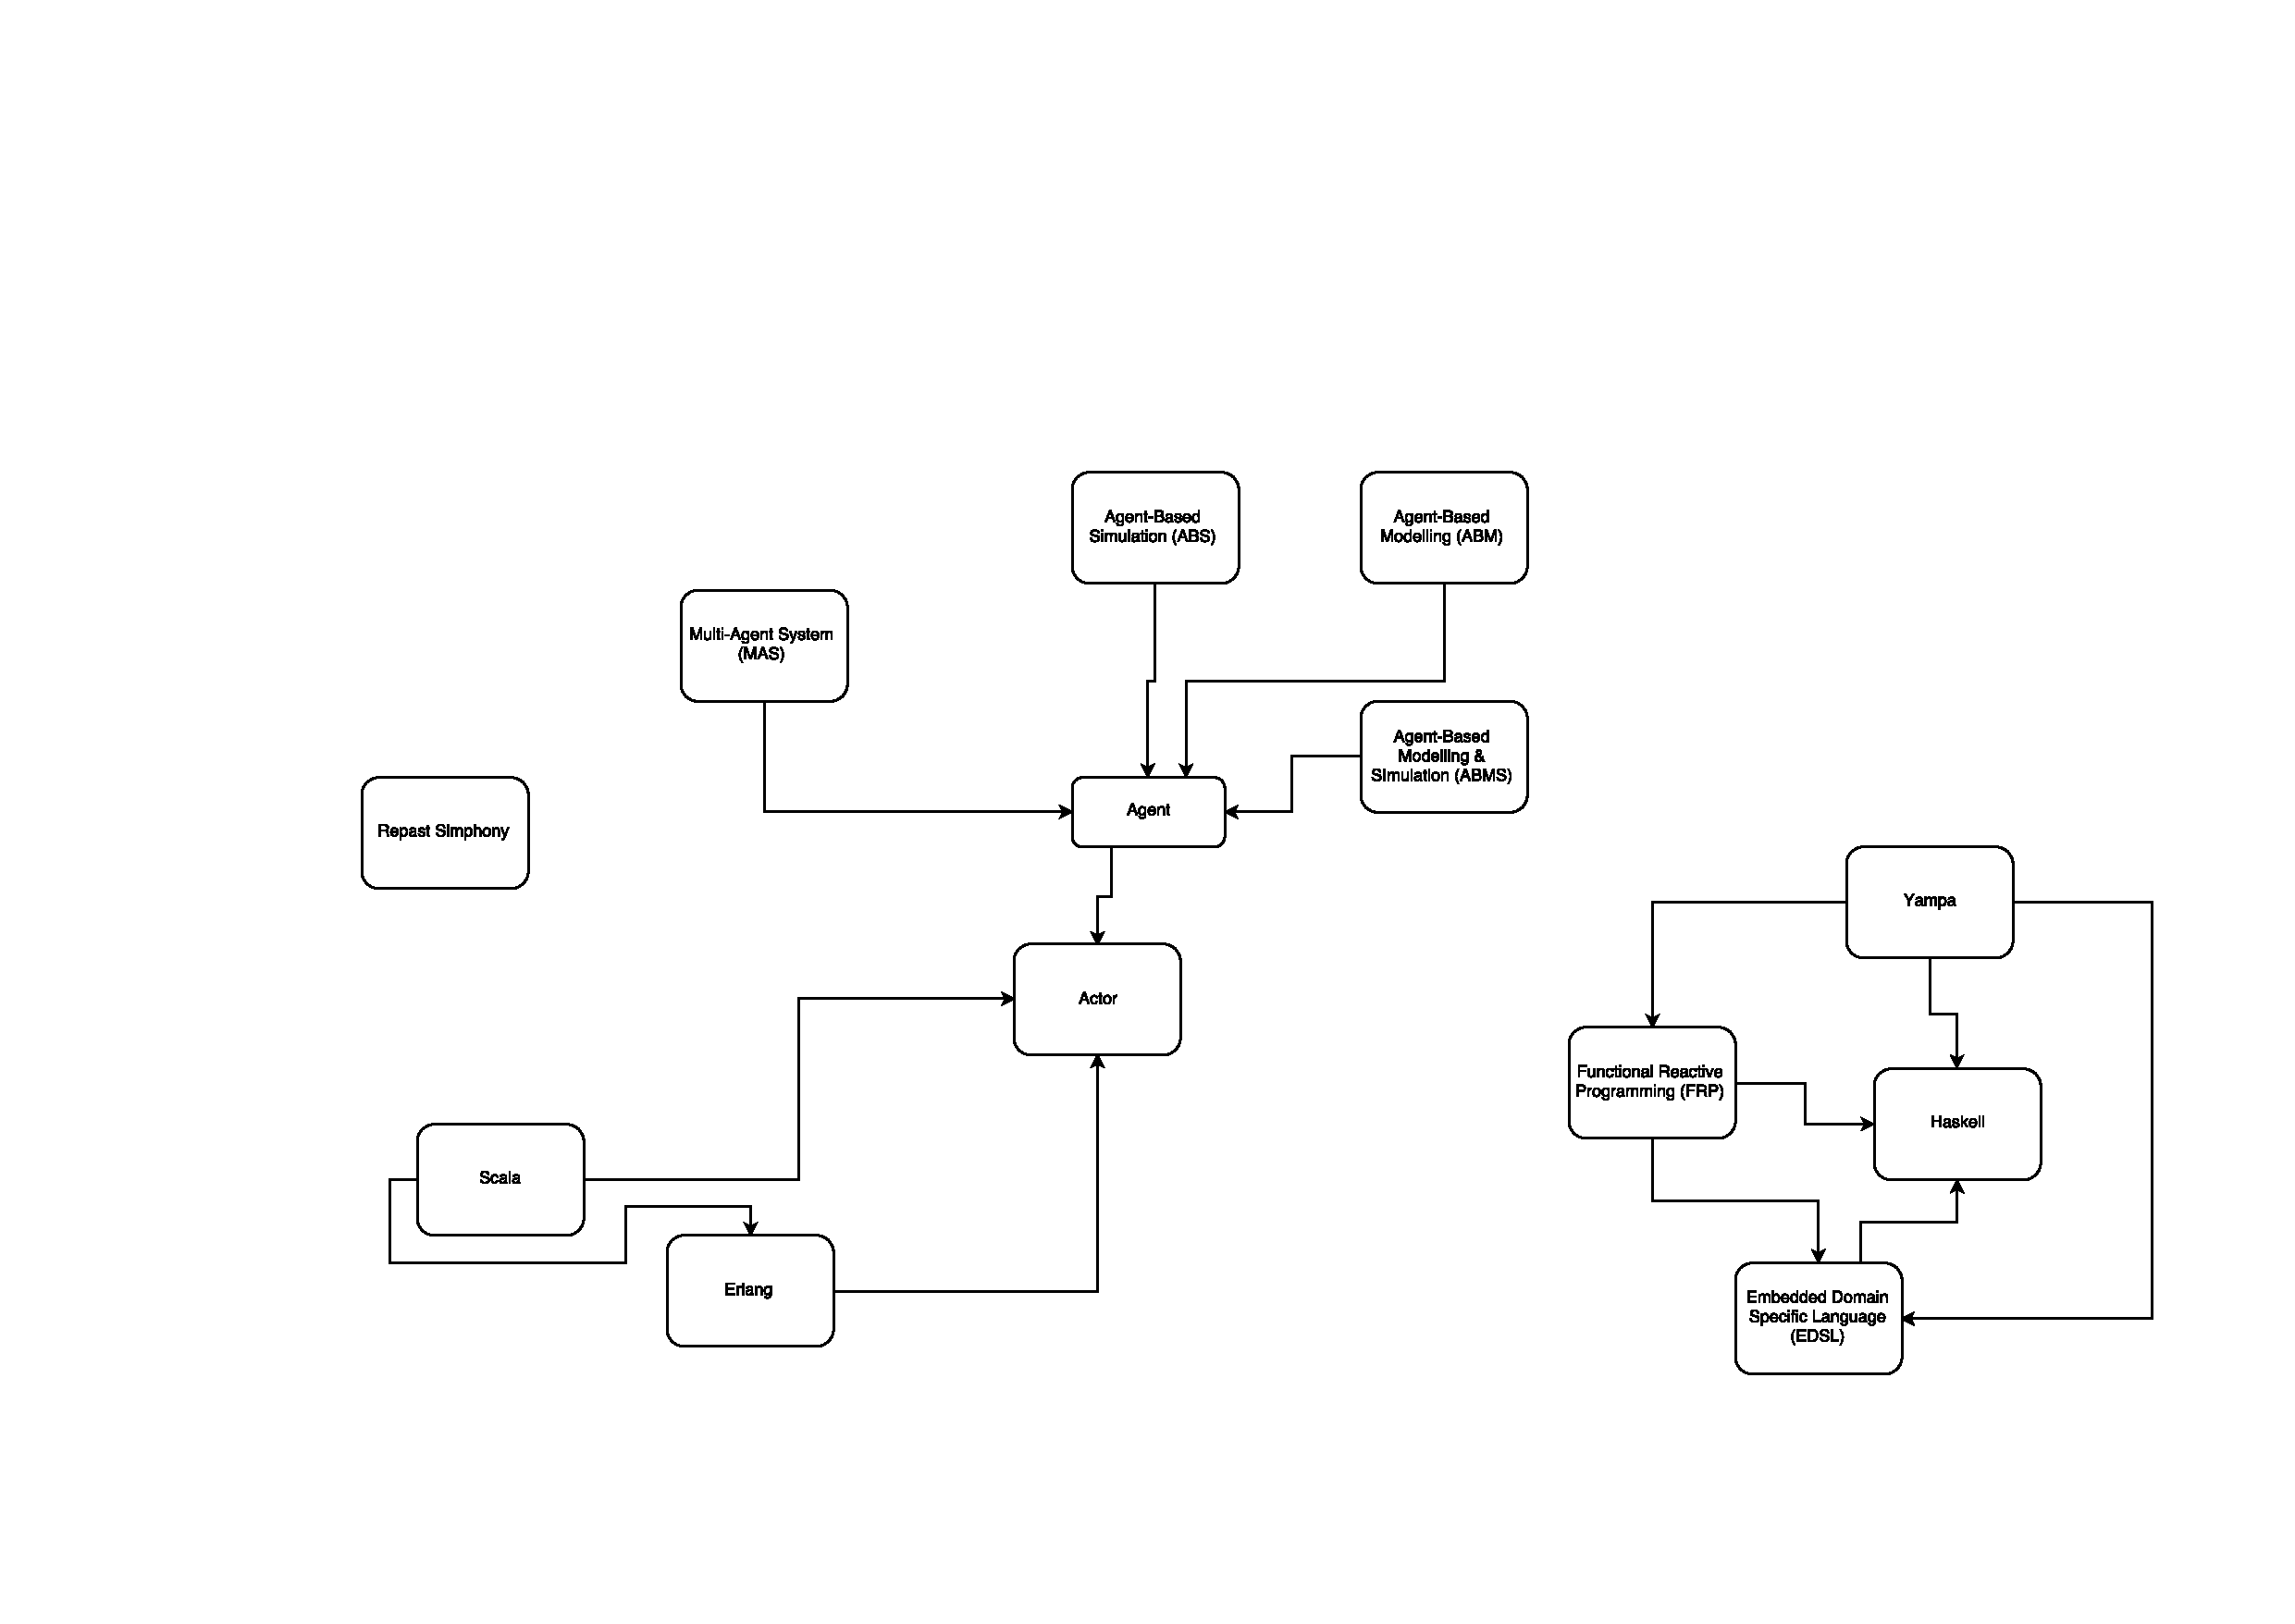
\includepdf[pages=-]{./poster/connections.pdf}

%	\begin{figure}
%		\label{fig:gantt}
%  		\caption{Gantt-Chart for remaining PhD}
%  		\centering
%  		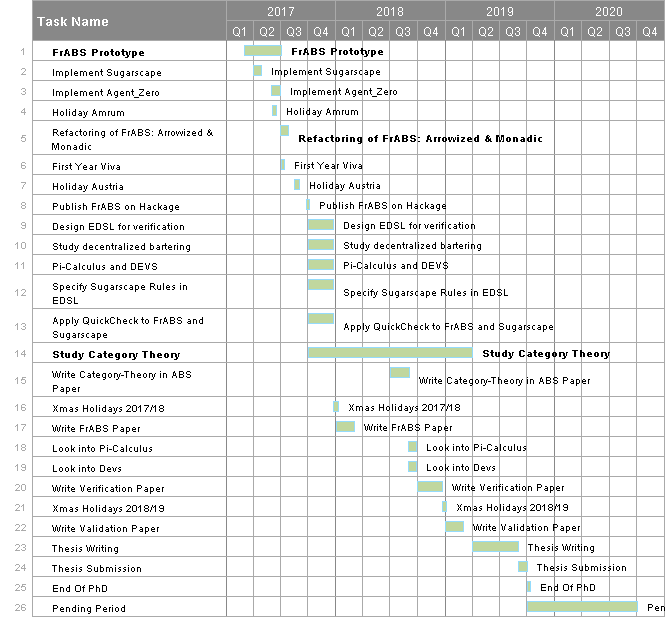
\includegraphics[width=1.2\textwidth]{./charts/gantt.png}
%	\end{figure}
\end{landscape}

\end{document}
